%\documentclass[11pt]{report}
\documentclass[11pt]{ucscthesis}
\usepackage{amssymb}
\usepackage{epsfig}
\usepackage{latexsym}
\usepackage{epsf}
\usepackage{xspace}
\usepackage{comment}
\usepackage{makeidx}
\usepackage{multicol}
%\usepackage{longtable}
%%%%%%%Luca's packages%%%%%

%\usepackage{epic}
%\usepackage{eepic}
\usepackage{luca}
\usepackage{vaibhav}
\usepackage{ds}
\usepackage{mocha}
%%%%%%%%%%%%%%%%%%%%%%%%%%%

%These we need as we would probably change the margins...
%\setlength{\textwidth}{14truecm}  %original is 12.2
%\setlength{\textheight}{21.5truecm}  %original is 19.3
%\setlength{\topmargin}{1.25in}
\setlength{\leftmargin}{-1.25in}

\makeindex

\title{ \chai - A Tool For Synchronous Interfaces}
\author{Vaibhav Bhandari}
%Computer Science and Engineering Department \\
%University of California, Santa Cruz \\
%{\tt vaibhav@cse.ucsc.edu} \\
%{\tt http://www.cse.ucsc.edu/\(\sim\)vaibhav}\\
%}

\degreeyear{2003}
\degreemonth{December}
\degree{Master of Science}
\numberofmembers{3}
\chair{Professor Luca de Alfaro}
\committeememberone{Professor Jim Whitehead}
\committeemembertwo{Professor Scott Brandt}
\field{Computer Science}
\campus{Santa Cruz}

\begin{document}
\pagenumbering{roman}
\maketitle
\copyrightpage
%\newpage
\tableofcontents
\listoffigures
\listoftables

\begin{acknowledgements}
\chapter*{Acknowledgements}
I would like to take this opportunity to thank my mentor
\textbf{Prof. Luca de Alfaro} for his constant support and
supervision during the course of this thesis.

\end{acknowledgements}
\clearpage
\pagenumbering{arabic}
\section{Introduction}
We describe a new interactive verification environment called \mocha
for the modular verification of heterogeneous systems.
\mocha differs from many existing model checkers in three significant ways:

\begin{itemize}
\vitem 
  For modeling, we replace unstructured state-transition graphs with
  the heterogeneous modeling framework of {\it reactive modules}
  \cite{Modules}.  The definition of reactive modules is inspired by
  formalisms such as Unity \cite{ChandyMisra88}, 
  I/O automata \cite{Lynch}, and Esterel
  \cite{BerryGonthier88}, and allows complex forms of interaction
  between components within a single transition.  Reactive modules provide a
  semantic glue that allows the formal embedding and interaction of
  components with different characteristics.  Some modules may be
  synchronous, others asynchronous, some may represent hardware,
  others software, some may be speed-independent, others
  time-critical.

\vitem
  For requirement specification, we replace the system-level specification 
  languages of linear and branching temporal logics \cite{Pnueli77,CE81}
  with the module-level specification language of 
  {\it Alternating Temporal Logic} (ATL) \cite{ATL}.
  In ATL, both cooperative and adversarial relationships between modules 
  can be expressed.
  For example, it is possible to specify that a module can attain a 
  goal regardless of how the environment of the module behaves.
%  Unlike system requirements, module requirements can be modified and 
%  reverified individually whenever the corresponding modules are changed.  

\vitem 
   For the verification of complex systems, \mocha supports a range of
   {\em compositional and hierarchical verification methodologies}.
   For this purpose, reactive modules provide assume-guarantee rules 
   \cite{HQR98} and abstraction operators \cite{TACAS98};
   \mocha provides algorithms for automatic refinement checking, and 
   will provide a proof editor that manages the decomposition of 
   verification tasks into subtasks.

% we complement model checking with
%  automated refinement checking for Reactive Modules.  Reactive
%  Modules is designed to capture the modularity of system designs in
%  such a way that the systems can be verified compositionally and
%  hierarchically. It has been proved that many {\em assume-guarantee}
%  rules are sound under this framework.

%  The refinement checking problem can be simplified
%  using the compositional and assume-guarantee rules.
%  To support hierarchical design at different levels
%  of abstraction and to aid the decomposition of verification tasks,
\end{itemize}

%\mypar


%The input language of \mocha is a readable variant of Reactive
%Modules. The following functionalities are currently being supported:

\noindent
In this paper, we describe the toolkit \mocha in which the
proposed approach is being implemented.  The input language of \mocha
is a machine readable variant of reactive modules.
The following functionalities are currently being supported:

\begin{itemize}
\vitem
Simulation, including games between the user and the simulator

\vitem
Enumerative and symbolic invariant checking and error-trace generation

\vitem
Compositional refinement checking

\vitem
ATL model checking 

\vitem
Reachability analysis of real-time systems
\end{itemize}

\noindent
\mocha is intended as a vehicle for the development of new
verification algorithms and approaches.  It adopts a software
architecture similar to \vis \cite{VIS96} , a symbolic model-checking
tool from UC Berkeley.  Written in C with Tcl/Tk and Tix
\cite{tix-http}, \mocha can be easily extended in two ways: designers
and application developers can customize their application or design
their own graphical user interface by writing Tcl scripts; algorithm
developers and researchers can develop new verification algorithms by
writing C code, or assembling any verification packages through C
interfaces.  For instance, \mocha incorporates the \vis packages
for image computation and multi-valued function manipulation, as well
as various BDD packages, to provide state-of-the-art verification
techniques.

%\begin{figure}[t]
%%\begin{center}
%%\centerline{\psfig{figure=mocha-sd1.ps,height=3in}}
%\centerline{\epsfysize250pt\epsfbox{mocha-sd.ps}}
%%\end{center}
%\end{figure}


\chapter {Interface Methodology}
\section{??}
\section{Witness modules for refinement checking}
\section{Abstraction modules}
\section{Assume-guarantee reasoning}

\chapter{\chai}
This chapter starts with an introduction to {\mocha } \cite{Mo98}, on
which \chai \ is built. It is then is followed by a tutorial on
modelling and verification using {\chai}. Towards the end of the
chapter the details of {\im}, their implementation, and their usage are
presented.

\section{The Starting Point- \mocha} \chai \ is based on {\mocha },
it extends the functionality of \mocha \ and adds an input
language to suit interfaces.

\mocha \ is an interactive environment for modular verification of
%<<<<<<< chai.tex
%heterogeneous systems of digital components, including those that
%are synchronous or asynchronous, speed-independent or real-time,
%and finite or infinite state. {\mocha } relies on the modelling
%framework of reactive modules unlike traditional use of state
%transition graphs. Its input language is machine readable variant
%of reactive modules. In \chai \ we extend \rm \ to interface
%modules as explained in next chapter.
%=======
heterogeneous systems of digital components.  \mocha \ relies on the
modelling framework of reactive modules. Its input language is a machine
readable variant of reactive modules. In \chai \ we extend \rm \ to
interface modules as explained in the next chapter.
%>>>>>>> 1.19

%\section{Mocha}
%Some lines on mocha implementation


%This section describes Mocha in summary detail.
\mocha \ supports the following functionalities \cite{mochaman}:
\begin{itemize}
\item \textbf{System specification} in the language of Reactive
Modules. Reactive Modules allow the formal specification of
heterogeneous systems with synchronous, asynchronous, and
real-time components. Reactive Modules support modular and
hierarchical structuring and reasoning principles.

\item \textbf{System execution} by randomized, user-guided, or
mixed-mode trace generation. In mixed-mode trace generation, the
user plays a game against \mocha \ and guides the execution of
some modules, while \mocha \ controls the execution of other
modules.

\item \textbf{Requirement specification} in Alternating Temporal
Logic \cite{ATL}. The logic ATL allows the formal specification of
requirements that refer to collaborative as well as adversarial
relationships between modules. The popular logic CTL
(Computational Tree Logic) \cite{ATL} is a sublanguage of ATL.

\item \textbf{Requirement verification} by ATL model checking. The
symbolic model checker in both implementations is based on BDD
engines developed by the UC Berkeley VIS project \cite{VIS96}. For
invariant checking, \mocha \ supports both symbolic and
enumerative search.

\item \textbf{Implementation verification} by checking trace
containment between implementation and specification modules.
\mocha \ supports containment checking if the specification module
has no hidden state, and simulation checking otherwise. For
decomposing proofs, \mocha \ supports an assume-guarantee
principle.

\item \textbf{Reachability analysis} of real-time systems.
\end{itemize}

In \mocha\ the basic structuring units, or the molecules of a
system, are {\em reactive modules} \cite{RM96journal}. The modules have
a well-defined interface given by a set of \emph{external (or
input)} variables and a set of {\em interface (or output)}
variables. A module may also have a set of {\em private}
variables. All variables are typed, and \mocha \ supports a
standard set of finite and infinite types, such as boolean and
integers. A module is built from \emph{atoms}, each grouping
together a set of \emph{controlled} (interface or private)
variables with exclusive updating rights.

\emph{Updating} is defined by two nondeterministic guarded
commands: an \emph{initialization} command and an \emph{update}
command. These commands decide the new value of the controlled
variable by picking up the guarded commands non-deterministically.
In these commands unprimed variables, such as $x$, refer to the
old value of the corresponding variable, and primed variables,
such as $x'$, refer to the new value of the corresponding
variable.  An atom is said to \emph{await} another atom if its
initialization or update commands refer to primed variables that
are controlled by the other atom.

The variables change their values over time in a sequence of
\emph{rounds}. The first round consists of the execution of the
initialization command of each atom, and the subsequent rounds
consist of the execution of the update command of each atom,  in
an order consistent with the await dependencies. A round of an
atom is therefore a \emph{subround} of the module. If no guard of
the update command is enabled, then the atom idles,
i.e., the values of the variables do not change.  %If the update
%command of an atom has a branch with a true guard and no updating
%action, then it may at any time either take a transition or idle.
%Such an atom is called \emph{lazy}, and is useful for modelling
%asynchronous interaction.
%
%%%Use a better example ?
%For example, consider the specification of a village telephone
%system that contains four telephones. The specification consists
%of two modules: the first one models the environment, i.e., the
%users, and the second one models the system. A phone is either
%on-hook or off-hook, and the module {\tt UserSpec}
%nondeterministically toggles at most one telephone between on-hook
%and off-hook.
%\begin{example}{}
%\begin{verbatim}
%type hookType is {on, off} module UserSpec is
%  interface h1,h2,h3,h4: hookType;
%lazy atom ToggleHook
%  controls h1,h2,h3,h4
%  reads h1,h2,h3,h4
%  init
%    [] true -> h1' := on; h2' := on; ...
%  update
%    [] h1 = on -> h1' := off;
%    [] h1 = off -> h1' := on;
%    ...
%  endatom
%endmodule
%\end{verbatim}
%\end{example}

Modules can be \emph{composed} if they have disjoint sets of
interface variables, and their union of atom sets does not contain
a circular await dependency. Given a specification {\tt
SystemSpec} of a system and model of user behavior as {\tt
UserSpec}, specification module {\tt Spec} is defined as:
\vspace*{-2ex}
\begin{footnotesize}
\begin{verbatim}
module Spec is UserSpec || SystemSpec
\end{verbatim}
\end{footnotesize}
\vspace*{-2ex} For encapsulation \rem{} allows the {\em hiding} of
interface variables, and for instantiation it allows the {\em
renaming} of interface and external variables. Hiding and parallel
composition permit hierarchical descriptions of complex systems.

\section{Tutorial Introduction to \chai}
%This section starts with a quick taste of chai.
Chai will be available for free public download from
\cite{getchai}. It requires the GLU BDD package and Tcl7.2. The
installation instructions and relevant notes are available at
\cite{getchai}.

\subsection{Modelling with \chai}
Consider modelling the 2-bit down counter shown in Figure
\ref{fig:downcounter} as an interface module. The counter counts
from 3 to 0 on its normal run. Whenever the reset is high the
counter resets itself to start down counting from 3. Thus we have
the input, reset and outputs, counting bits $b0$ and $b1$.

To model this downcounter as an interface we should first
understand the input assumption and output guarantee of the
system. In case of the downcounter, the input assumption is fairly
trivial, the input \emph{reset} can be either 1 or 0. So we choose
it to be non- deterministic denoted as \texttt{nondet}. The output
guarantee is that counter counts from $3 \rightarrow 2 \rightarrow
1 \rightarrow 0 \rightarrow 3$ when it is not reset and on being
reset starts counting from 3. We represent this as guarded
commands. If the state of counter (reset,b1,b0) is (0,1,0) then in
the next state it should move to zero if the reset stays low i.e
(0,0,0) low so we have a guarded command as shown below. Note that
the control variables (b1, b0) take the values (false, true) only
if the guard on left of right arrow is true.
\begin{verbatim}
       [] ~reset &  b1 & ~b0 -> b1' := false; b0' := true
\end{verbatim}

Figure \ref{fig:modeldowncounter} shows the interface module for
the down counter shown in Figure \ref{fig:downcounter}.

\begin{figure}[htbp]
\centering
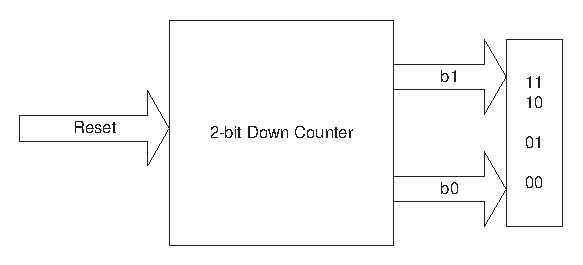
\includegraphics[width=4in]{figs/downcounter}
\caption{A 2-bit Down Counter}
\label{fig:downcounter}
\end{figure}

\begin{figure}[h]
\centering
\input{egs/downcounter.intf}
\caption{A 2-bit Down Counter Modelled As An Interface Module}
\label{fig:modeldowncounter}
\end{figure}

\subsection{Running \chai}
All the interface module definitions have to be entered into a
single file named typically with the suffix .intf; in our case,
(say) this file is downcounter.intf (Figure
\ref{fig:modeldowncounter}). \chai \ is invoked by typing {\tt
chai} at the shell prompt.

\begin{verbatim}
kala 6> chai
Welcome to CHAI 1.0
Please report any problems to dvl@cse.ucsc.edu
chai 1.0 >
\end{verbatim}

\noindent The interface is read and parsed with the {\tt
read\_intf} command. As shown below \chai \  displays the names of
the modules that were successfully parsed. In the case of a parse
error, an appropriate message is displayed.

\begin{verbatim}
kala 68> chai
Welcome to CHAI 1.0
Please report any problems to dvl@cse.ucsc.edu
chai 1.0 > read_intf downcounter.intf
...
DEBUG Interface Created: downcounter
chai 1.0 >
\end{verbatim}

\chai \ provides many methods and tools for verifying the
correctness of a design: execution (i.e., simulation), invariant
checking, refinement checking, ATL model checking, interface
composition. Interface composition being the distinguishing
feature of \chai \ we detail it here, the rest of the features are
described in \cite{mochaman}.

The command for interface composition is {\tt compose\_intf}.
\begin{verbatim}
chai 1.0 > compose_intf
Usage: compose_intf <outIntf> <Intf1> <Intf2>
\end{verbatim}

\noindent It checks if the interfaces {\tt Intf1} and {\tt Intf2}
can be composed as a new interface {\tt outIntf}. When we run this
command on interface downcounter (Figure \ref{fig:downcounter} )
and a dual output gate (Figure \ref{fig:gate}).
\begin{figure}[h]
\centering
\input{egs/gate.intf}
\caption{A Simple Gate} \label{fig:gate}
\end{figure}
The composition gives a compatible interface as following \chai \
session shows.
\begin{verbatim}
chai 1.0 > read_intf downcounter.intf
...
chai 1.0 > read_intf gate.intf
...
chai 1.0 > compose_intf GC gate downcounter
Interfaces gate and downcounter are compatible.
\end{verbatim}


\section{Interface Modules}
\im\ consist of input and output variables controlled by input and
output atoms. In this section we look at them in detail.

\subsection{Variables}
The state of an interface module is described by a set of {\em
state variables}. They are in turn partitioned into sets of {\em
input\/} and {\em output\/} variables. The \emph{input variables}
represent inputs to the interface, their value can be read, but
not changed, by the interface module. The input variables are
denoted by an \textbf{inputs vars:} clause. The \emph{output
variables} represent outputs of the interface, and their value can
be changed (and read) by the interface module. The output
variables are denoted by \textbf{output vars:} clause.

Consider the description of the downcounter as an interface
(Figure \ref{fig:modeldowncounter}). The variable are declared in
the beginning as:
\begin{verbatim}
  input vars:  reset: bool;
  output vars: b0: bool; b1: bool;
\end{verbatim}
Here reset is defined as an input variable of type boolean, while
b0 and b1 are defined as output variables of type boolean.

\subsection{Intialization and Transitions}
The variables in an interface module have to be initialized at
system reset and assigned new values at each clock tick. A
variable can be assigned a new value only by the atom which
\emph{controls} it. The input and output variables achieve this
through \emph{input atoms} and \emph{output atoms} respectively.

\textbf{Input atoms} describe the initialization and update of
input variables. The input atom transition relations model the
design assumptions about the inputs provided by the environment
and a set of {\em initial inputs\/} specify the desired initial
condition of the environment. For example the input variable reset
of downcounter is described with an input atom as follows:
\begin{verbatim}
input atom controls reset
  init
       [] true -> reset' := nondet
  update
       [] true -> reset' := nondet
  endatom
endinterface
\end{verbatim}
Here the guarded commands are marked by [], the keyword nondet
gives a value to the controlled variable non-deterministically.

\textbf{Output atoms }describe the initialization and update of
output variables. The transition relations in output atom model
the possible changes of output variables describing the behavior
of the module. The initial outputs specify the initial conditions
of the module. For example the output variables $b0,b1$ of
downcounter are described with an output atom as follows:
\begin{verbatim}
output atom controls b0, b1 reads b0, b1, reset
  init
       [] true -> b0' := true; b1' := true;
  update
       []  reset             -> b1' := true;  b0' := true
       [] ~reset &  b1 &  b0 -> b1' := true;  b0' := false
       [] ~reset &  b1 & ~b0 -> b1' := false; b0' := true
       [] ~reset & ~b1 &  b0 -> b1' := false; b0' := false
       [] ~reset & ~b1 & ~b0 -> b1' := true;  b0' := true
  endatom
\end{verbatim}
Here the output variables (b0,b1) are controlled by the atom and
they are assigned values based on guards managed by predicates
involving b0, b1 and reset.

\subsection{Syntax}
Any {\tt .intf} file contains one interface definition. The
interface definition has the syntax described in Figure
\ref{fig:interfacesyntax}. The \chai \ environment knows the
interface by \emph{interface-name}. Each state variable in an
interface is controlled by one and only one atom. The \emph{input
atoms} describe the input assumptions while the \emph{output
atoms} state the output guarantees.

\begin{figure}
\centering
\begin{verbatim}
                    interface <interface-name>
                        input vars: <input-list>
                        output vars: <output-list>

                        [input | output] <atom>
                        ...
                        [input | output] <atom>
                    endinterface
\end{verbatim}
\caption{Syntax of Interface Module} \label{fig:interfacesyntax}
\end{figure}

\subsection{Semantics}
The semantics of an interface module is essentially a simple game
between the module and its environment.

The behavior of an interface module consists of an infinite
sequence of states starting from an initial state (trace).
Starting with initial state each successive state is generated by
the module and by its environment. The modules chooses the new
values of the output variables according to the output transition
relation, while the environment must choose the new values of the
input variables according to the input transition relation.

If the module is able to fulfill all its output guarantees even
for a single set of environment variables then the module is said
to be compatible with its environment.

\subsection{Implementation}
%parser -> reactive modules -> fsm -> composed -> interfaces
The formalism of interface modules as described here is
implemented in {\chai }. The parser of \mocha \ was changed to
accommodate the input language of interface modules. The parser
splits the interfaces into input assumption and output guarantee
\rm \ which in turn are converted in to finite state machines
(FSM) represented as binary decision diagrams. The FSMs are then
composed into a single interface. The resulting interface is
referred in the \chai \ environment by the name it had in its
interface definition file.

Composition and compatibility checking for interfaces as presented
in section \ref{sec:algo} is implemented by extending the CUDD BDD
package and the VIS BDD manipulation package \cite{VIS96} in the
{\chai } environment. Using the techniques explained in section
\ref{sec:algo}, the size (number of BDD variables) of the
interfaces that \chai \ is able to check for compatibility, and
compose, is roughly equivalent to the size of the models that
\mocha \cite{Mo98} can verify with respect to safety properties.

\section{Chai Operations}
This section presents various commands available to work in the
\chai \ design and verification environment. There are different
data structures on which one can work at different levels of
granularity and different amount of control. Here we present a
summary of commands which each relevant data structure or
abstraction can handle. The detailed list of \chai \ commands and
functions can be found online at \cite{getchai}.

\subsection{ Interfaces}
Interface modules can be read in the \chai \ environment by the
command \texttt{read\_intf}. Two interfaces can be composed by the
\texttt{compose\_intf} command. The levels of various variables in
the module can be known by poking it with \texttt{print\_levels}.

\subsection{Reactive Modules}
Reactive modules can be read in the \chai \ environment by using
the commands \texttt{read\_module}. Two reactive modules can be
composed by using the \texttt{compose} command. A module can be
renamed by using the \texttt{ren} directive and a new instance of
it can be created using the \texttt{let} command. One can see the
atoms comprising a module by using the \texttt{show\_atoms}
command.

\subsection{BDDs and  FSMs}
 Binary decision diagrams are at the bottom of data
structure hierarchy. They form the core of the implementation. MDD
(multivariate decision diagrams) and FSMs (finite state machines)
follow next.

A module can be converted in to a FSM using the commands
\texttt{fsm}. An interface can be made from FSM representations by
using the commands \texttt{make\_intf}.

A dump of BDDs from a module file can be obtained by using the
commands \texttt{dump\_bdd} in a module. Various operations like
\texttt{not,and,or} can be performed directly on BDDs. The truth
value of a BDD can be checked using \texttt{true} command.

\subsection{Invariants}
Invariants can be read in the \chai \ environment by the
\texttt{read\_inv} command. Invariants in alternating temporal
logic are read using \texttt{atl\_read}. To check wether a module
satisfies an invariant one can use the command \texttt{inv\_check}
on an instance of module and the invariant.

\subsection{Summary of Important Commands}
A handy list of important \chai \ commands is presented below:
\begin{itemize}
    \item \textbf{read\_intf}. This commands reads and validates an interface module description from the specified file.
    \item \textbf{sl\_make\_intf}. This command given two modules, one describing the input evolution, the other describing the output evolution, creates a single new interface module that combines the two.
    \item \textbf{sl\_make\_intf\_out}. This command creates an interface having only an output portion (with no input
    assumptions).
    \item \textbf{sl\_compose\_intf}. This command given two interfaces, composes them and checks if they are compatible. If they are not compatible, says so. If they are compatible, says so, and returns the composition.
    \item \textbf{sl\_check\_intf\_ref}. This commands given two interfaces intf1 and intf2, checks whether intf2 is a refinement of intf1.
    \item \textbf{sl\_print\_intf}. This command prints an interface on the console.
    \item \textbf{sl\_copy}. This command makes a copy of an interface and references it by the name specified by the commandline parameter.
    \item \textbf{sl\_compose}. This command composes two FSMs even if they share controlled variables, and references the composition by the name specified by the commandline parameter.
    \item \textbf{sl\_reach\_histonly}. This command computes the set of reachable states, projected onto the history variables only.
\end{itemize}


%\section{Issues}
%Bad States and Control problem.

\chapter{Interfaces for Hardware Design}
One of the goals of \chai \ is to formally verify hardware designs
%<<<<<<< mv2rm.tex
%at the Register Transfer Logic (RTL) level. {\chai } has a Binary
%=======
at the Register Transfer Logic (RTL) level. {\chai} has a Binary
%>>>>>>> 1.19
Decision Diagram (BDD) based formal verification engine and has
algorithms to compose and verify designs. A developer can use
these algorithms to formally verify existing hardware designs.
Tools for converting existing component based hardware designs to
the \chai \ environment are required to be able to provide such a
comprehensive test bed for component-based design verification
algorithms and methodologies. This chapter describes the
conversion of hardware designs coded in Verilog, Esterel or VHDL
to Interface Modules, as summarized in Figure \ref{fig:hdl2intf}.

\begin{figure}[htbp]
\centering
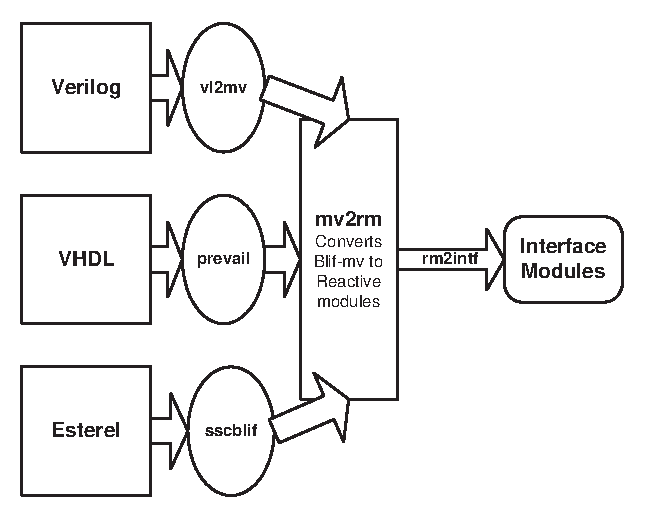
\includegraphics[width=4in]{figs/hdl2intf}
\caption{Converting Hardware Description Languages to Interfaces}
\label{fig:hdl2intf}
\end{figure}

\section{HDL to BLIF-MV}
Verilog to \mv \ conversion is possible by the tool vl2mv
\cite{vl2mv}. VHDL to \mv \ conversion can be achieved by the tool
prevail \cite{PREVAIL} while Esterel has a back-end SSCBlif
\cite{sscblif} to output code in \mv \ format. Thus, \mv \ is a
rich intermediate format.

\section{{\mv }}
\mv \ is an acronym for Berkeley Logic Interchange Format ---
Multivariate. It is successor of BLIF, and it primarily adds
non-determinism. The \mv \ format is designed to represent
non-deterministic sequential systems in hierarchical fashion. A
system can be composed of interacting sequential systems, each of
which can be again described as a collection of communicating
sequential systems. In {\mv }, there is an implicit assumption
that the whole system is clocked by a single global clock,
although the clock is never declared in {\mv }.

We implemented a tool to convert a \mv \ representation of a
design to reactive modules. The next two sections describe the tool
\mvrm \ and the translation process.

\subsection{MV2RM}
\begin{figure}[htbp]
\resizebox{3in}{!}
{\includegraphics[0,0][3in,3in]{figs/car}}
\caption{Pedestrian Crossing} \label{fig:piclights}
\end{figure}

Figure \ref{fig:piclights} illustrates a simple daily life
scenario of a pedestrian crossing. Here a simple traffic light
%<<<<<<< mv2rm.tex
%controller manages both the car traffic lights and the pedestrian
%=======
controller manages the car traffic lights and the pedestrian
%>>>>>>> 1.19
lights. Figure \ref{fig:pedlight} presents the example encoded in
{\mv}. When the \emph{CarSignal} is asserted and Mr. Bean pushes
\emph{Button} to cross the street then the \emph{ControlLogic}
de-asserts the \emph{CarSignal} at next clock-tick. When
\emph{CarSignal} is de-asserted the \emph{PedestrianSignal} gets
asserted. Finally, now Mr. Bean is able to cross the road!

The left column in Figure \ref{fig:pedlight} is the {\mv } model
\cite{b2m} and the right column is translation to {\rm } done by
{\mvrm }.

\begin{figure}
\centering
\includegraphics[1,0][7in,8in]{figs/modelLights}
%\input{egs/lights.mv}
%\hspace{4em}
%\input{egs/lights.rm}
\caption{Pedestrian Light Controller in BLIF-MV and {\rm}}
\label{fig:pedlight}
\end{figure}

Figure \ref{fig:mv2rmarch} shows the architecture of \mvrm . The
file {\tt lights.mv} is fed to the lexer of {\mvrm }. The
translation is two-pass. {\mvrm } is implemented in function
language OCAML \cite{ocaml}.

In pass one the \textbf{sub-circuit analyzer} parses the input
models {\mv } to analyze the parameters of the subcircuits used to
make an appropriate hide variable list when the model is converted
in to a {\rm }.

In pass two the \textbf{parser} goes through all the \mv \
constructs to make an abstract syntax tree. The validation of
input is done in this phase. At the end of the pass the code
generator runs over the abstract syntax tree to emit \rm \ code.

\begin{figure}[htbp]
\centering \resizebox{4in}{!}{
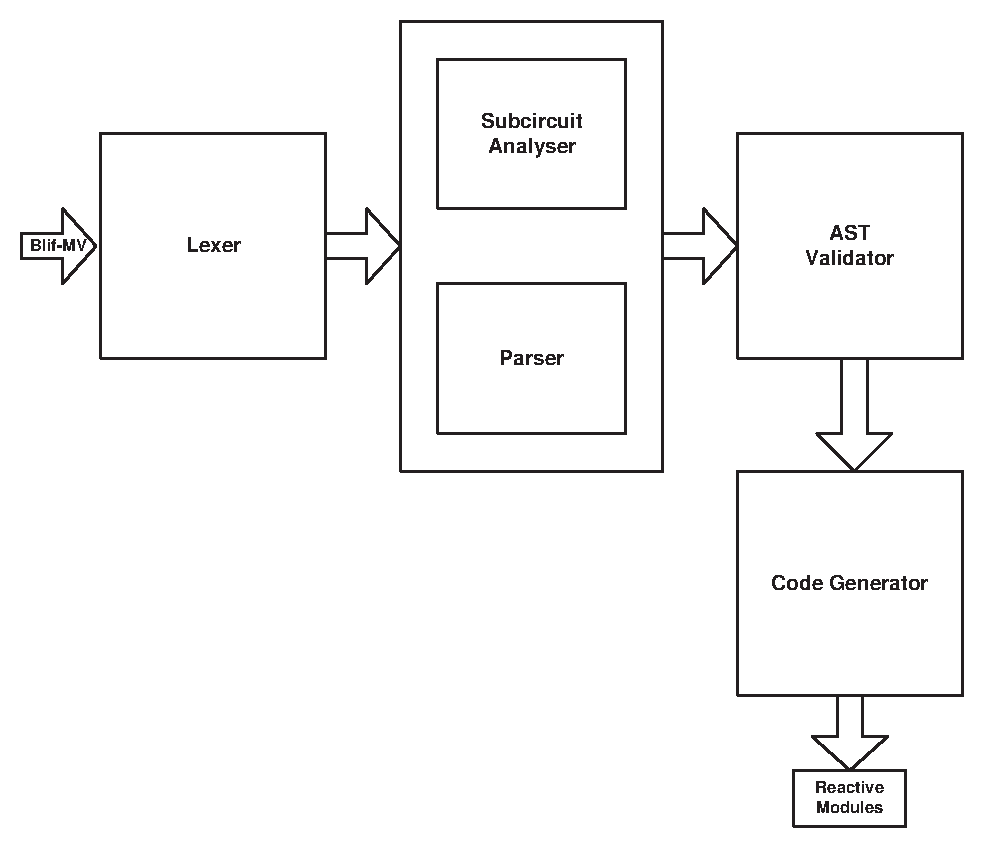
\includegraphics[width=4in,bb= 20 20 600 400]{figs/mv2rmarch}}
\caption{Architecture of {\mvrm} } \label{fig:mv2rmarch}
\end{figure}


\section{Translating {\mv } to {\rm }}
In this section we describe the translation logic used by
{\mvrm}. Each important construct of {\mv } is described with a
relevant example and the corresponding strategy of conversion is
detailed.  The Full BNF grammar of {\mv } is given in the appendix and
the documentation of the OCAML implementation of \mvrm \ will be at
\cite{mv2rmdoc}.

\begin{figure}[h]
\begin{center}
\begin{tabular}{|l|l|}
  \hline
  {\mv } & {\rm }\\
  \hline
  model & module \\
  \hline
  inputs & interface \\
  \hline
  outputs & external \\
  \hline
  undefined var & private \\
  \hline
  table & atom (awaited)\\
  \hline
  reset & atom \\
  \hline
  latch & atom (read)\\
  \hline
  subckt & composition \\
  \hline
\end{tabular}
\end{center}
\caption{Mapping of {\mv } constructs to {\rm }}
\label{tab:mapping}
\end{figure}

\subsection{Multi-valued Variables}
A multi-valued variable is a variable that can take a finite
number of values. There are two classes of multi-valued variables.
The class of {\em enumerative variables} consists of variables
whose domain is the $n$ integers $\{0,\ldots,n-1\}$.

\begin{verbatim}
.mv <variable-name-list> <number-of-values>
\end{verbatim}

The second class are {\em symbolic variables}, which can take a
set of arbitrary values. Symbolic variables are declared as
follows.
%All references to multi-valued variables in {\tt .table} and {\tt .reset}
%should be done after their declarations by {\tt .mv} construct.

\begin{verbatim}
.mv <variable-name-list> <number-of-values> <value-list>
\end{verbatim}

{\rm } have multi-valued variables. Table \ref{tab:mv} shows how
enumerative and symbolic variables are translated. {\rm } also
have typed variables which can be used to represent symbolic
variables.

\begin{table}
\begin{center}
\begin{tabular}{lll}
  %\hline
 .mv signal 3 & $\Rightarrow$ & signal: (0..2)\\
  %\hline
 .mv signal 3 \ STOP READY2GO GO & $\Rightarrow$ & signal: \{STOP,
  READY2GO, GO\}\\
   % \hline
\end{tabular}
\end{center}
\caption{Multivalued Variables Translated}
\label{tab:mv}
\end{table}

\subsection{Tables}
A table is an abstract representation of a physical gate. A table
is driven by inputs and generates outputs as defined by its
functionality. Although a real gate generates an output
deterministically depending on what inputs are supplied, tables in
{\mv } can represent non-deterministic behaviors as well. The
functionality of the table is described as a symbolic relation,
i.e the table enumerates symbolically all the valid combination of
values among the inputs and the outputs. A table without input
represents a constant generator. If the table allows more than one
value for its output, then the table is a {\em nondeterministic}
constant generator, which we call {\em pseudo input}. Tables are
declared in the following way.

\begin{verbatim}
.table <in-1> <in-2> ... <in-n> -> <out-1> <out-2>... <out-m>
<relation>
...
<relation>
\end{verbatim}

The table is translated as an \emph{ atom }in {\rm }. The input
variables are read fresh for each clock tick, i.e they are
\emph{awaited} and the output variables are controlled.

 A {\em relation} of \mv \ is a white-space separated non-null list of
$n+m$ strings, giving a valid combination of values among inputs
and outputs. The $i$-th string in a relation specifies a set of
values for the $i$-th variable in the input/output declaration of
{\tt .table}. A relation of \mv \ is translated as a
\emph{guarded command} of {\rm }. In each update round the values
of controlled variables (outputs in tables) are based on the
guarded commands (relations).

The {\tt .default} construct of \mv \ is used to define a default
output for the input patterns not specified in the given relation.
A default construct \mv \ is translated as a default guarded
command of {\rm }.

Table \ref{table:tabl} shows a \mv \ .table snippet from Figure
\ref{fig:pedlight} translated into {\rm }. Note that the atom has
awaited variables.
%\begin{verbatim}
%.table PresentSignal Button -> NextSignal
%.default 1
%1 1 0
%.end
%\end{verbatim}
%
%It is translated as the following atom.
%\begin{verbatim}
% atom
%   controls  NextSignal
%   awaits  PresentSignal , Button
%     init update
%     []  PresentSignal' = 1  &
%       Button' = 1  -> NextSignal':= 0
%     [] default -> NextSignal':=1
% endatom
%\end{verbatim}

\begin{table*}
\input{egs/table.mv}
\hspace{3em}
\input{egs/table.rm}
\caption{Tables translated}
\label{table:tabl}
\end{table*}
%
%Let us consider the following example.
%
%\begin{verbatim}
%.mv x,y 4
%.table x -> y
%!2 {1-3} - 0 2 (0,3)
%\end{verbatim}
%
%The relation specified in this table is: $[(0,1,3) \times (1,2,3)]
%\cup [(0,1,2,3) \times (0)] \cup [(2) \times (0,3)]$.

%Tables are represented as atoms in \rm \ and the relations of a
%table are correspondingly compiled as relations of the atoms over
%guarded commands. Each output variable can be controlled by only
%one atoms so while translating a table this constraint is always
%checked.

\subsection{Latches and Reset Tables}
A latch models a storage element, which retains the value of the
input at the last clock tick. A latch has \emph{only one} input
and output. Every latch has to be initialized by a  \emph{reset}
statement. A latch is allowed to have more than one initial value,
in which case the latch takes an initial value
non-deterministically from the specified values. Thus a latch can
be seen as a multi-valued flip-flop with possibly multiple initial
states. The reset statement specifies the values \emph{latched
variables} can take when the system is reset.

A latch is declared as follows:
\begin{verbatim}
.latch <latch-input> <latch-output>
\end{verbatim}

The reset statement for a latch is as follows:
\begin{verbatim}
.reset <option-reset-input> latch_output
<reset-in-0> <value-0>
...
\end{verbatim}

The {\mvrm } parser goes through the input file combines the {\bf
latch} and {\bf reset }statements for a particular variable. The
\emph{latch-output} variable is controlled by the atom and
initialized according to the relations in the reset statement. It
is updated to the value of \emph{latch-input}. Note that the value
of \emph{latch-input} is \textbf{read} by the atom and not
awaited, implying that it does not wait for the variable to be
update in current round bu t rather picks its value from the last
round. Table \ref{tab:lr} illustrates the conversion.

%\begin{table}
%\begin{center}
%\begin{tabular}{|l|l|}
%  \hline
%.latch Tmp CarSignal &  atom \\
%.reset CarSignal     &  {\ }controls  CarSignal \\
%0                    &  {\ }\textbf{reads}  Tmp \\
%1                    &  {\  }init \\
%                     &  {\   } []  true  \-> CarSignal':= 1 \\
%                     &  {\   } []  true  \-> CarSignal':= 0 \\
%                     &  {\  } update \\
%                     &  {\   }[]  true \->  CarSignal':=Tmp \\
%                     &  endatom \\
%\hline
%\end{tabular}
%\end{center}
%\caption{Latch and Reset Statements Translated} \label{tab:mv}
%\end{table}
\begin{table}
\input{egs/latch.mv}
\hspace{3em}
\input{egs/latch.rm}
\caption{Latch and Reset Statements Translated} \label{tab:lr}
\end{table}

\subsection{Models}
{\tt .model} is the prime construct of {\mv } used to define a
basic component of a hierarchical system.

Any {\mv } file contains one or more model definitions. In case of
multiple models in a single file the first model is considered to
the {\tt root} model or the model having {\tt .root} construct in
second line of its definition . A model looks like Figure
\ref{fig:model}.
\begin{figure}[h]
\begin{verbatim}
                        .model <model-name>
                        .inputs <input-list>
                        .outputs <output-list>
                        <command>
                        ...
                        <command>
                        .end
\end{verbatim}
\caption{{Blif-MV} model syntax} \label{fig:model}
\end{figure}

\begin{itemize}
\item {\em model-name} is a string by which the model is referred
in the system. The equivalent construct to a model in \rm \ is a
module. Each model is abstracted as a module. Table
\ref{tab:model} illustrates the conversion.

\item {\em input-list} is a white-space separated list of strings
(terminated by the end of the line) giving the formal input
terminals for the model being declared. If this is the root model,
then signals can be identified as the primary inputs of this
system. The input variables are mapped as  \emph{external}
variables while translating to {\rm }.

\item {\em output-list} is a white-space separated list of strings
(terminated by the end of the line) giving the formal output
terminals for the model being declared. If this is the root model,
then signals can be identified as the primary output of this
system. The input variables are mapped as \emph{interface}
variables while translating to {\rm }.

\item {\em command} is one of {\tt .mv}, {\tt .table}, {\tt
.latch}, {\tt .reset} and {\tt .subckt}, which defines the
detailed functionality of the model. Translation of {\tt .subckt}
is described in next section while rest are detailed in previous
sections. Undeclared variables are mapped as private variables
while translating to {\rm  }.
\end{itemize}

\begin{table}
\input{egs/model.mv}
\hspace{3em}
\input{egs/model.rm}
\caption{{\tt .model} translated} \label{tab:model}
\end{table}


\subsection{Subcircuits}
In a model, another model can be instantiated as a subcircuit
using the {\tt .subckt} construct. It is the contruct which
enables hierarchical composition in {\mv}.

\begin{verbatim}
.subckt <model-name> <instance-name> <formal-actual-list>
\end{verbatim}

This construct instantiates a reference model {\em model-name} as
an instance {\em instance-name} in the current model. {\em
formal-actual-list} specifies the association between each formal
variable in {\em model-name} and its corresponding actual variable
in the current model. Formal variables are declared in the
reference model, while actual variables are variables declared in
the current model. {\em formal-actual-list} is a list of
assignments separated by a white space. The declaration of {\em
formal-actual-list} is of form:

\begin{verbatim}
formal-1 = actual-1 formal-2 = actual-2 ... formal-n = actual-n
\end{verbatim}

The {\tt .subckt} construct is replaced by composition construct
of {\rm }. A model M with subckts A1..An is represented as $M =
a\_M \parallel A1 \parallel A2 \ldots \parallel An $, here a\_M is
the base model M without the subcircuits.

Special processing is performed for the actual parameters passed
to the subcircuits in the base model. To do subcircuit analysis
and special processing we maintain a modelTab, which is a hash
table of models, hashed by the modelname and containing the 3
lists, inlist, outlist, subcktlist of the model. If the actual
passed parameter from the base model is an output and the
associated formal parameter in subcircuit is an output in the
subcircuit then it is made an input in the base model (a\_module).
This is because on composition it will be an output in $ module =
a\_module \parallel subckt$. If the actual passed parameter from
the base model is a private variable and associated formal
variable is an output in the subciruit then it is made an input in
the base model (a\_module) and added to a hidelist, this is
because on composition it will be output in $ module = a\_module
\parallel subckt$ but it should be hidden from the world by $
module = hide \ hidelist \in \ a\_module \parallel subckt $.

Consider the translation shown in table \ref{tab:subckt}, and note
that the private variable {\tt Tmp} in model {\tt Lights} is added
to hidelist and is made an output (external) variable in the base
model a\_Lights.

\begin{table}
\input{egs/subckt.mv}
\hspace{3em}
\input{egs/subckt.rm}
\caption{Partial {\tt .subckt} Translation}
\label{tab:subckt}
\end{table}

\section{{\rm } to Interfaces modules}
We have implemented a tiny tool {\tt rms2intf} which integrates
the input assumption and output guarantee reactive modules to form
an interface module.

\begin{verbatim}
kala 39> rms2intf -h

Usage: rms2intf inputAssumption.rm outputGuarantee.rm
\end{verbatim}

Figure \ref{fig:counterrms} shows the input assumption of a 2-bit
down counter in left hand column and the output guarantee in the
right hand column. All the atoms in input assumptions weaved as
input atoms in the interface representation and the output
guarantee atoms become output atoms. Figure \ref{fig:counterintf}
shows the interface output from {\tt rms2intf}. Note that instead
of interface and external we term the variables as output and
input.

\begin{figure}
\input{egs/counterI.rm}
\hspace{4em}
\input{egs/counterO.rm}
\caption{Reactive Modules Representing a Down Counter}
\label{fig:counterrms}
\end{figure}

\begin{figure}
\centering
\input{egs/counterIO.intf}
\caption{Interface Representation of Down Counter by {\tt
rms2intf}} \label{fig:counterintf}
\end{figure}

The hardware design extracted in above fashion can be input in the
{\chai } environment in the form of reactive modules or interface
modules as illustrated by Figure \ref{fig:chairmintf}

\begin{figure}
\begin{verbatim}
kala 100> chai
Welcome to CHAI 1.0
Please report any problems to dvl@cse.ucsc.edu
chai 1.0 > read_module counterO.rm
Module counterO is composed and checked in.
parse successful.
chai 1.0 > read_intf counterIO.intf
...
Done..
DEBUG PrsReadIntfCmd :  counterIO.intf.I
Module counterOI is composed and checked in. parse successful.
Module counterOO is composed and checked in. parse successful.
...
DEBUG Interface Created: counterIO
chai 1.0 > exit
Thank you for using CHAI 1.0
\end{verbatim}
\caption{ HDLs in {\chai}}
\label{fig:chairmintf}
\end{figure}

\chapter{Conclusion and Future Work}
\section{Future Work}


\appendix
\chapter{BLIF-MV BNF}
\begin{minipage}[h]{2in}
\scriptsize
\begin{verbatim}
main:
    models TokEOF
;
models:
    model models
  |
;
model:
      head decl body \
      TokEnd TokEOL
;
head:
    TokModel TokVar TokEOL
;
decl:
      vdecl
  |
;
vdecl:
      vdecl input
  | input
  | vdecl output
  | output
;
\end{verbatim}
\end{minipage}

\hspace{4em}
\begin{minipage}[h]{2in}
\scriptsize
\begin{verbatim}
iovals:
      TokVar iovals
  | TokVar
;
body:
   table body
  | subckt body
  | mv  body
  | reset  body
  | latch body
  |
;
table:
      TokTable tabvars \
      TokEOL relations

;
mv:
      TokMV mvvars TokVal \
      values TokEOL
;
mvvars:
      TokVar COMMA mvvars
  | TokVar
;
\end{verbatim}
\end{minipage}

\clearpage
\begin{minipage}[t]{2in}
\scriptsize
\begin{verbatim}
subckt:
      TokSubckt TokVar TokVar param_passing TokEOL

;

param_passing:
    formal_actual param_passing
  |
;

formal_actual:
      TokVar ASSIGN TokVar


;

latch:
      TokLatch TokVar TokVar TokEOL

;

tabvars:
      inList ARROW outList { add_in_list ($1);
                 add_out_list ($3)}
  |   TokTabVar inList

  | TokTabVar

inList:
    TokTabVar inList
  | TokTabVar
  | {[]}
;

outList:
    TokTabVar outList
  | TokTabVar
;

relations:
      vdefault relations
  | relation relations
  | {}
;

vdefault:
      TokTabDef valList TokEOL
;

relation:
      valList TokEOL { ($1) }
;

valList:
      valb valList { ([$1]@($2)) }
  | valb { [$1] }
;

valb:
      TokTabVal
  |   TokTabVar
  | ASSIGN  TokTabVar
  | HYPHEN
  | LBRACE TokTabVal HYPHEN TokTabVal RBRACE
  | LPAREN vals RPAREN
  | NOT valb
;

vals:
      TokTabVal COMMA vals
  | TokTabVal
;
\end{verbatim}
\end{minipage}

\hspace{4em}
\begin{minipage}[t]{2in}
\scriptsize
\begin{verbatim}
values:
      TokVar values
  | TokVal values
  |
;
reset:
  TokReset tabvars \
  TokEOL relations
;
relations:
      vdefault relations
  | relation relations
  |
;
vdefault:
  TokTabDef valList TokEOL
;
relation:
      valList TokEOL
;
valList:
      valb valList
  | valb
;
valb:
      TokTabVal
  |   TokTabVar
  | ASSIGN  TokTabVar
  | HYPHEN
  | LBRACE TokTabVal HYPHEN
        TokTabVal RBRACE
  | LPAREN vals RPAREN
  | NOT valb
;
vals:
      TokTabVal COMMA vals
  | TokTabVal
;
\end{verbatim}
\end{minipage}


\chapter{Grammar Of Interface Modules}
\begin{verbatim}
interface <interface-name>
    input vars: <input-list>
    output vars: <output-list>

    [input | output] <atom>
    ...
    [input | output] <atom>
endinterface
\end{verbatim}
\nopagebreak

\bibliographystyle{alpha}
\bibliography{thesis}
\end{document}
